\section{Definicja anomalii (obserwacji odstającej)}
Obserwacje odstające to punkty, które nie odpowiadają wzorcowi w zbiorze danych. Barnett i Lewis definiują obserwację odstającą następująco: ,,Obserwacja odstająca jest to obserwacja, której obecność jest różna od pozostałych obserwacji'' \cite{barnett1984outliers}. Rysunek \ref{fig:anomalia} obrazuje przykład obserwacji odstających (anomalii) dla dwuwymiarowego zbioru danych. Zbiór danych posiada obszar wzorcowy {$N_1$}, większość punktów leży wewnątrz tego obszaru. Punkty wystarczająco oddalone od obszaru $N_1$: $o_1$, $o_2$, $o_3$ -- sklasyfikowane są jako obserwacje odstające (anomalie).
\begin{figure}
    \centering
    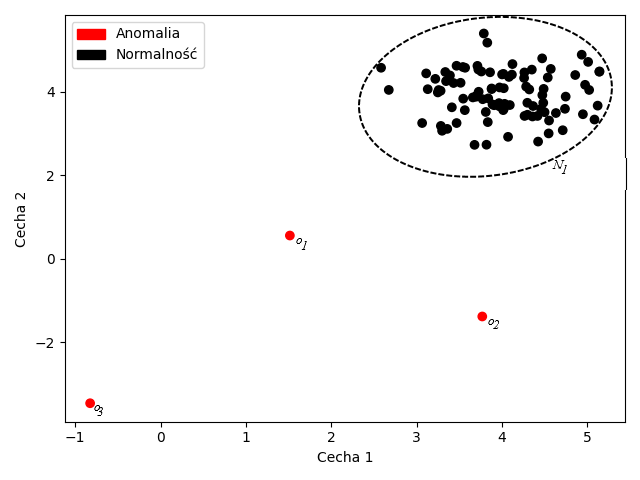
\includegraphics[width=.5\textwidth]{chapters/istniejace/images/anomalia.png}
    \caption{Prosty przykład anomalii w dwuwymiarowym zbiorze danych}
    \label{fig:anomalia}
\end{figure}

\section{Zadanie detekcji anomalii}
W pracy rozważamy uczenie nienadzorowane na zbiorze $N$ punktów $x_1,...,x_N$ każdy punkt jest d-wymiarowym wektorem liczb rzeczywistych. Zbiór danych składa się z obserwacji poprawnych i anomalnych, jednakże zbiór nie posiada wektora $y_1,..,y_N$ -- klasyfikującego obserwację do obserwacji poprawnych lub anomalnych. Zadaniem jest wykrycie punktów anomalnych w danym zbiorze. Zadanie detekcji anomalii jest zadaniem klasyfikacji jednoklasowej. 

\section{Różnice w podejściu detekcji anomalii}

\subsection{Wykrywanie anomalii lokalnych a globalnych}
\label{sub:loc_glob}
Podejście dotyczy wyboru zakresu zbioru jako zbioru odniesienia dla rozpatrywania odstawania danej obserwacji. Główne podejścia to: podejście globalne oraz lokalne. Rysunek \ref{fig:anomalie_glob_lok} obrazuje prosty zbiór dwuwymiarowy z dwoma klastrami poprawnych obserwacji: $c_1$ i $c_2$. Dla punktów $x_1 $ oraz $x_2$ klasyfikacja jako anomalie jest możliwa wizualnie. Oba te punkty są znacząco oddalone od gęstych obszarów obserwacji. Są to anomalie globalne. Rozpatrując wszystkie obserwacje zbioru punkt $x_3$ mógłby być uznany za poprawną obserwację należącą do klastra $c_2$, jednak kiedy rozpatrzymy podzbiór punktów w sąsiedztwie klastra $c_2$ (zbiór odniesienia), punkt $x_3$ może być uznany za anomalię. Jest to przykład anomalii lokalnej. Zatem anomalia lokalna jest to obserwacja, której wystarczające odchylenie od normy jest w obszarze najbliższego sąsiedztwa (zbioru odniesienia). 
\begin{itemize}
    \item Podejście globalne 
    \begin{itemize}
        \item Zbiór odniesienia obejmuje wszystkie obserwacje
        \item Założenie o istnieniu jeden prawidłowego mechanizmu generującego normalne punkty.
        \item Problem: inne obserwacje odstające mogą również występować w zbiorze danych zaburzając rezultat detekcji.
    \end{itemize}
    \item Podejście lokalne 
    \begin{itemize}
        \item Zbiór odniesienia jest podzbiorem całego zbioru
        \item Brak założenia o liczbie mechanizmów generujących.
        \item Problem: wybór odpowiedniego podzbioru
    \end{itemize}
\end{itemize}

% \begin{figure}[]
%   \centering
%   \begin{minipage}{0.4\textwidth}
%     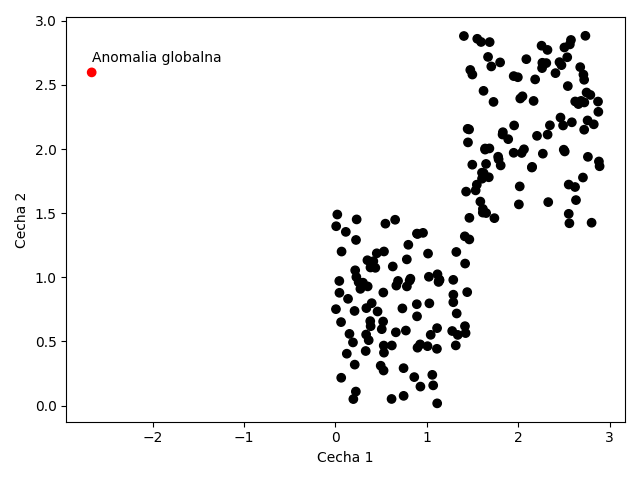
\includegraphics[width=\textwidth]{chapters/istniejace/images/anomalia_globalna.png}
%     \caption{Przykład anomalii globalnej}
%     \label{fig:global}
%   \end{minipage}
%   \hfill
%   \begin{minipage}{0.4\textwidth}
%     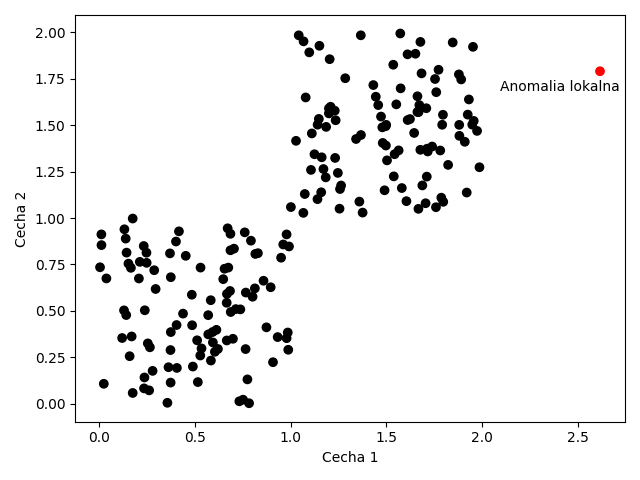
\includegraphics[width=\textwidth]{chapters/istniejace/images/anomalia_lokalna.png}
%     \caption{Przykład anomalii lokalnej }
%     % A comperative evaluation ma lepszy obraz
%     \label{fig:local}
%   \end{minipage}
% \end{figure}
\begin{figure}
    \centering
    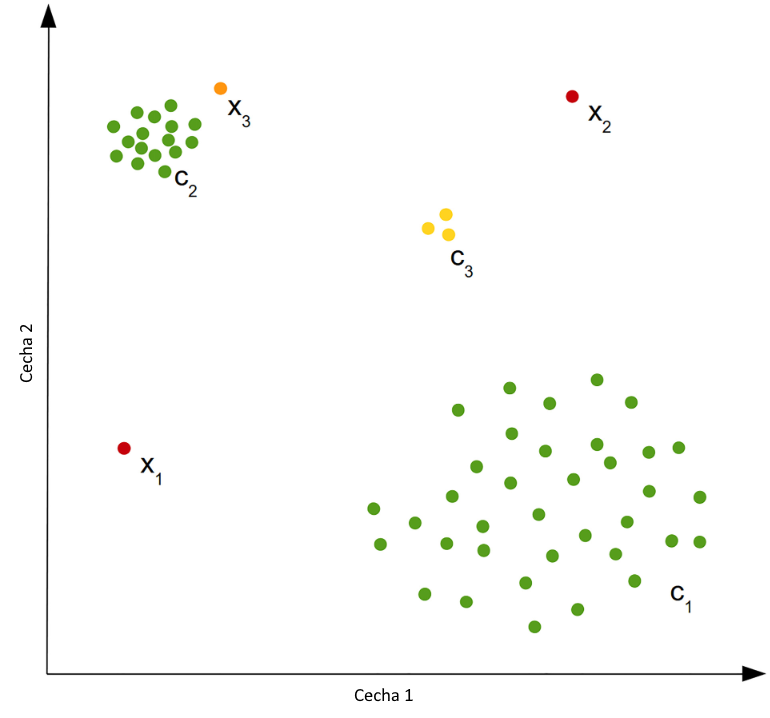
\includegraphics[width=.5\textwidth]{chapters/istniejace/images/mikro_cluste.png}
    \caption{Przykład anomalii globalnych ($x_1, x_2$), lokalnej $x_3$ oraz mikro klastra $c_3$ \cite{goldstein2016comparative}}
    \label{fig:anomalie_glob_lok}
\end{figure}

\subsection{Wynik metody}
\label{sec:score}
Ważnym aspektem dla metody wykrywania anomalii jest sposób oceny każdej obserwacji. Dane wyjściowe metody mogą przypisywać obserwacji wartość anomalności na dwa warianty:
\begin{itemize}
    \item binarny: przypisanie obserwacji etykiety normalnej obserwacji lub anomalnej
    \item ciągły: dla każdej obserwacji obliczany jest wynik anomalności np. prawdopodobieństwo obserwacji jako anomalii
\end{itemize}
Wiele podejść opartych na przypisywaniu wyniku anomalności skupia się na wyznaczeniu grupy n-obserwacji o najwyższym wyniku (parametr n często podawany jest przez użytkownika np. wartość kontaminacji). Również z tego podejścia można za pomocą np. progu wyniku anomalności otrzymać binarną etykietę obserwacji dzięki temu osoba analizująca dane może dostosować próg dla danej dziedziny.

Podejście oparte na ciągłym wyniku anomalności punktu przydatne jest w rozważaniu mikro klastrów, czyli małych regularnych klastrów. Rysunek \ref{fig:anomalie_glob_lok} obrazuje mikro klaster $c_3$. Algorytm detekcji anomalii powinien przypisać punktom klastra wartość większą od normalnych obserwacji oraz mniejszą od anomalii globalnych. Ten przykład pokazuje, że podejście przypisywania ciągłej wartości anomalności punktu jest podejściem bardziej użytecznym od binarnej klasyfikacji. Jak również problematyczność klasyfikacji.

\subsection{Rodzaje anomalii}
% Punktowe, collective i contextual - można wszystko z punktowych które są dominujące w unsupervised detection
W detekcji anomalii wyróżnia się trzy rodzaje anomalii: anomalie punktowe, anomalie zgrupowane, anomalie kontekstowe.
Większość dostępnych algorytmów detekcji anomalii dla uczenia nienadzorowanego opiera się na wykrywaniu pojedynczych przypadków anomalnych punktów. Detekcja anomalii zgrupowanych została przedstawiona na rysunku \ref{fig:anomalie_glob_lok} i opisana w sekcji \ref{sec:score} -- mikro klaster $c_3$.
Anomalie kontekstowe są to anomalie najczęściej spotykane w szeregach czasowych. Dotyczy to punktów, które mogą być uznane za poprawne obserwacje jednak rozpatrywane w kontekście charakteru zbioru danych zostaną uznane za anomalie. Aby zobrazować weźmy przykład pomiaru temperatury w skali roku we Wrocławiu. Temperatura 25$^{\circ}$C wydaje się być poprawnym odczytem temperatury, jednak w kontekście miesiące np. stycznia. Tak wysoka temperatura jest anomalią.

Szczęśliwie można wykorzystać algorytmy detekcji anomalii punktowych do wyrywania anomalii zgrupowanych i kontekstowych. Dla zademonstrowanego przykładu pomiary temperatury kontekst (miesiąc) może być uwzględniony jako cecha obserwacji. Jednakże dla bardziej złożonych zastosowań może wystąpić potrzeba przekształcenia zadanie detekcji anomalii kontekstowych w zadanie detekcji punktowych. 

Przekształcenie z zadania detekcji anomalii zgrupowanych do detekcji anomalii punktowych wymaga wiedzy na temat zbioru danych. Generuje się nowy zbiór danych reprezentujący cechy w inny sposób z wykorzystaniem korelacji, agregacji oraz grupowania \cite{goldstein2014behavior}. 

Detekcja różnych typów anomalii wymaga obróbki danych w celu zapewnienia poprawnego działania algorytmu detekcji. W pracy skupiono się na problemach detekcji anomalii punktowych bez potrzeby dodatkowego przekształcania danych.

% \subsection{Podejścia w konstrukcja metody detekcji anomalii} 
% \begin{itemize}
%     \item Parametryczna
%     \item Nieparametryczna
% \end{itemize}
% Przykład technik opisany szerzej w sekcji \ref{section:methods}

% \section{Przykłady podejść do zadania wykrywania anomalii}
% \label{section:methods}

% \begin{figure}
%     \centering
%     \includegraphics[width=\textwidth]{chapters/istniejace/images/TypyAlgorytmów(1).png}
%     \caption{Przykład nienadzorowanych algorytmów detekcji anomalii z rozdzieleniem na stosowane podejście }
%     \label{fig:typy}
% \end{figure}
% \subsection{Podejście statystyczne}
% Pierwsze badania anomalii oraz metod ich wykrywania polegały na modelowaniu statystycznym. Anomalie mogą zaburzać zadania: estymacji, predykcji czy klasyfikacji. Pojawienie się anomalii powoduje zmianę m.in. średniej z próby i wariancje. 
% \section{Główne metody detekcji anomalii}
% Dla zadania detekcji anomalii w celu doboru odpowiedniej metody należy na samym początku rozpatrzyć zbiór odniesienia (opisane w podsekcji \ref{sub:loc_glob}) oraz algorytm, który dokładnie modeluje dystrybucję danych. Większość algorytmów detekcji dla uczenia nienadzorowanego opartych jest na następujących metodach:
%     \subsection {Oparte na wiedzy statystycznej}
%     Podejście opiera się na idei zastosowania metod statystycznych w celu wykrycia anomalii.
%     \subsection {Oparte na metryce}
%     \subsection {Oparte na gęstości zbioru}
%     \subsection {Oparte na klasteryzacji}
%     \subsection {Oparte na łączeniu klasyfikatorów (zespół klasyfikatorów)}
%     \subsection {Oparte na sieciach neuronowych}

\section{Problematyka}
